% 01_Introduction
\chapter{Introduction}
\noindent InCroMAP is an application that is able to import processed microarray data from different platforms and perform gene-centric integration of those. It holds many novel analysis methods that allow, e.g., integrated pathway-based visualization, gene set enrichment across multiple platforms or integrated tabular views. InCroMAP can handle directly the following four platforms:

\begin{enumerate}
\item messenger RNA (mRNA) expression data
\item micro RNA (miRNA) expression data
\item protein and protein modification expression data
\item DNA methylation data
\end{enumerate}

InCroMAP is a high-level data analysis tool. This means that no low-level data processing methods (normalization, smoothing, etc.) are included in InCroMAP. The reader is referred to the R statistical computing language to perform low-level data processing for microarrays. But this also means that InCroMAP supports data from various microarray manufacturers. To import microarray data, InCroMAP just needs any gene identifier and some statistics, i.e. fold changes or p-values, for each probe. Therefore, it is also possible to use data from other platforms than the mentioned four. Please see the \hyperref[ch:faq]{FAQ} for more information on this.


Besides developing powerful analysis methods and visualization tools, we have put a huge amount of work to make InCroMAP as easy-to-use as possible. Therefore, InCroMAP already includes many pre-processed datasets and mapping files. This also includes, for example, integrated microRNA targets from different databases for multiple organisms or mapping files to convert different IDs to gene symbols.

The detailed list of features is very long and every feature is described in it's own section in more detail. The following is a list of the main features of InCroMAP:

\begin{itemize}
  \item Getting started:
  \begin{itemize}
  \item Read processed microarray data from tabular text files
  \item Manually import gene lists
  \item Show microRNA targets for human, rat or mouse, choosing one or multiples of the following databases:
  \begin{itemize}
    \item Experimentally verified
      \begin{itemize}
      \item miRecords
      \item miRTarBase
      \item TarBase
      \end{itemize}
    \item Predicted
      \begin{itemize}
      \item ElMMo
      \item DIANA � microT
      \item TargetScan
      \end{itemize}
  \end{itemize}
  \item Visualize KEGG Pathways
  \end{itemize}


  \item Single dataset analysis:
  \begin{itemize}
  \item Gene set enrichment analysis:
    \begin{itemize}
    \item KEGG Pathway enrichment
    \item Gene Ontology (GO) enrichment
    \item Enrichments using any gene set from the Molecular Signatures Database (MSigDB)
    \end{itemize}
  \item Annotate targets of miRNAs
  \item Pathway-based visualization of any microarray data
  \item Locus-based visualization of DNA methylation data
%  \item \dots
  \end{itemize}

  \item Integrated, cross-platform analysis methods (using data from heterogeneous platforms):
  \begin{itemize}
    \item Data pairing (e.g., showing miRNA data together with mRNA targets)
    \item Gene-centered and expandable integrated tabular view of multiple platforms
    \item Integrated gene set enrichment analysis (enrichment across multiple platforms, same databases supported as mentioned before)
    \item Pathway based visualization of microarray data from four different platforms in one pathway
  \end{itemize}


  \item Pathway visualization features:
  \begin{itemize}
    \item Visualization of various KEGG pathways
    \item Highlighting enriched genes from a pathway enrichment analysis directly in a visualized KEGG pathway
    \item Searching/Highlighting of genes/compounds, etc.
    \item Visualization of data directly in a pathway:
    \begin{itemize}
      \item Coloring pathway nodes according to an observation (e.g., mRNA fold change)
      \item Adding miRNA nodes with relevant targets to the pathway
      \item Coloring miRNA nodes
      \item Extending pathway-nodes to visualize expression data for various protein modifications
      \item Extending pathway-nodes to show the amount of differential methylation in gene promoters
      \item Showing corresponding observations/ expression values directly in the tooltip of pathway nodes
    \end{itemize}
    \item Inspecting locus-based DNA methylation regions for specific pathway genes
  \end{itemize}


  \item Application features:
  \begin{itemize}
    \item Easy-to-use and user-friendly
    \item All features are included in one graphical user interface
    \item Automatic detection of file formats and contents
    \item Customization of various options with the "Preferences" dialog
    \item Help available directly in the application
    \item Cross-linked pathway view (double-click nodes to get more info)
    \item Save and export everything (to multiple formats)
    \item Everything included (targets, mappings,...) and non-included data is downloaded automatically
    \item Multiple FDR correction methods included
    \item Application is available for download and also runs as Java WebStart
  \end{itemize}
\end{itemize}


%%%%%%%%%%%%%%%%%%%%%%%%%%%%%%%%%%
% 02_Installation
%%%%%%%%%%%%%%%%%%%%%%%%%%%%%%%%%%
\chapter{Installation}
InCroMAP comes as a Java JAR file. It can run out-of-the-box on all systems where a Java virtual machine is installed and does not require any further installations.

\section{Requirements}
\subsection{Software}
InCroMAP is entirely written in Java\TTra and runs on any operating system where a suitable Java Virtual Machine (JDK version 1.6 or newer) is installed. See, for example, the Java SE download page\footnote{\url{http://www.oracle.com/technetwork/java/javase/downloads/index.html}
\label{fn:jvmldl}}.

\subsection{Hardware}
With at least 1\,GB main memory, you should be able to perform most tasks without any problem.
For large datasets, you should have at least 2\,GB of main memory. \newline
An active internet connection is required for most operations.

\section{Starting the application}
\label{startingTheProgram}
If you downloaded a ZIP-file, you need to unzip it before starting the application. Depending on your operating system, you should use the provided shell scripts for starting the application. This is \texttt{start.sh} for Linux or \texttt{start.bat} for Windows. On MAC OS, you have to create your own shortcut. You can start the application on all operating systems by typing

\begin{lstlisting}[language=bash,numbers=none]
java -jar -Xms128m -Xmx1024m InCroMAP.jar
\end{lstlisting}

\noindent on your command prompt. Please note that you might have to change \texttt{InCroMAP.jar} for the real name of the JAR-file, e.g., \texttt{InCroMAP1.2.0.jar}. In this example, a minimum of 128\,MB and a maximum of 1024\,MB of memory will be available for the program. In most cases, InCroMAP needs more than 128\,MB memory, so it might be convenient to create a shortcut and start the application with as much memory as available. If you have 2\,GB RAM, for example, you might want to start the application with the following command:

\begin{lstlisting}[language=bash,numbers=none]
java -Xms128m -Xmx1400M -jar InCroMAP.jar
\end{lstlisting}

For your convenience, we already created several start-scripts to run the application with as much memory as possible. How much memory you actually need strongly depends on the size of your input datasets.
%
\newline\newline \textbf{It is strongly recommended to start the program with at least 1\,GB memory (\texttt{-Xmx1G}).}\newline


\chapter{How to get started}
This chapter gives detailed information how to load data from various platforms into the InCroMAP application. The InCroMAP homepage provides example data and an additional screencast (i.e., short video tutorial) that shows how to open data and perform a first analysis with InCroMAP. This might be a good starting point for first time users.

\section{Prepare microarray data}
\label{ch:prepare}

First of all, make sure that your microarray data is in one of the required file formats. The application can read character separated value (CSV) files, which are mostly tab-separated tabular files with microarray data. To use EXCEL-data, you can simply open your EXCEL spreadsheet, click "File" and "Save as" and select "Tab-separated text file".
For nearly all data formats, the most important columns are your observations, which can be p-values or fold-changes, and one column with any gene identifier. Supported gene identifiers are gene symbols, NCBI Entrez Gene IDs, Ensembl gene IDs, RefSeq IDs or KEGG IDs. The fold-changes should be on a log scale (i.e., $log_2$ data) -- negative values represent downregulation, positive values upregulation and 0 is the base line for no expression change.

\emph{Note: InCroMAP can NOT process raw data. Please use only processed microarray data.}

\subsection{mRNA expression data}
As always, your file must be formatted as character (preferably tab) separated text file. Necessary columns are only one for the gene identifier and at least one column for your fold-changes or p-values.

Example:
\begin{lstlisting}[caption={Input file example for messenger RNA expression data},label={lst:input:mrna},numbers=none,captionpos=t,float=h]
Gene.Symbol	EntrezGene.ID	Ctnnb1_foldchange	Ras_foldchange
Copg        54161         0.17              0.64
Atp6v0d1    11972         0.04              -0.24
...         ...           ...               ...
\end{lstlisting}



\subsection{miRNA expression data}

MicroRNA datasets are required to be character separated text files. Besides columns with fold-changes or p-values, just one column, containing a systematic miRNA identifier, is required. The systematic name can refer to either the mature, or the pre-miRNA.


Example:
\begin{lstlisting}[caption={Input file example for micro RNA expression data},label={lst:input:mirna},numbers=none,captionpos=t,float=h]
Systematic_name Ctnnb1_foldchange Ras_foldchange
mmu-miR-96      1.45              7.21
mmu-let-7e      -0.72             0.46
...             ...               ...
\end{lstlisting}


\subsection{DNA methylation data}
InCroMAP can read any DNA methylation data with references to chromosomal locations. This can lead to huge datasets with up to single base pair resolution. To avoid having too much data, it is strongly recommended to summarize the data to bins of, e.g., $50bps$. Most microarray based DNA methylation datasets are already in a perfect format, because the probe length is mostly $50-75bps$.

All probes must somehow be mapped to genes. Therefore, in addition to the fold-change/p-value columns, at least one of the following three columns are required:
\begin{enumerate}
  \item An "Identifier" column that contains a direct (custom) mapping from every probe to a gene
  \item One "Chromosome" column and a "Probe position" column
  \item One column, containing chromosome and position as probe identifier (format: \texttt{CHR{chromosome}FS{position}}, e.g., \texttt{CHR12FS1234}). This is also used by some companies (e.g., Nimblegen) as probe identifier.
\end{enumerate}

In the later two cases, a dialog will appear that let's you choose how to map the data to the genome. Probes can either be mapped to gene bodies or promoter regions. In the later case, you can specify the region up-/ and downstream of a TSS.

\noindent\textbf{Note: it is always recommended to have chromosome and position information with your DNA methylation data. Without these information, creating genome-based plots is not possible!}

Example:
\begin{lstlisting}[caption={Input file example for DNA methylation data},label={lst:input:dnam},numbers=none,captionpos=t,float=h]
Gene               probe_start probe_end ProbeID          Ctnnb1_foldchange
ENSMUSG00000056912 100054458   100054515 CHR10FS100054458 0.08
ENSMUSG00000056912 100053768   100053817 CHR10FS100053768 0.04
ENSMUSG00000046567 100052169   100052221 CHR10FS100052169 0.08
...                ...         ...       ...              ...
\end{lstlisting}


\subsection{Protein modification expression data}

Protein expression datasets, as all other datasets, require a gene-identifier and columns with fold-changes or p-values. Furthermore, it is strongly recommended having a column, indicating the modification of the current protein (phosphorylation, cleavage, acetylation, methylation, etc). This is customized for, e.g., phosphoprotein datasets. Nevertheless, the modification column is optional. Thus, one can simply read protein expression datasets by just specifying an identifier and the observation columns.

Example:
\begin{lstlisting}[caption={Input file example for protein modification expression data},label={lst:input:protein},numbers=none,captionpos=t,float=h]
Analyte_ID  Gene_Symbol Modification EntrezGene Ctnnb1_foldchange
AKT1        AKT1        basic        11651      0.24
AKT1_P-S473 AKT1        P-S473       11651      -0.34
PRKAA1      PRKAA1      basic        105787     0.07
...         ...         ...          ...        ...
\end{lstlisting}

The modification column indicates, if and how the protein is modified and at which site. For example, "P-S473" indicates a phosphorylation of the serine 473 site. The term "basic" refers to the unmodified protein. These modifications prevent InCroMAP from mixing different values of the same protein, that originate from different protein modifications (example input data may originate from reverse-phase-protein-arrays, e.g., from Zeptosense). But for simple protein expression data (without modification expression information), one can simply omit the modification column.

\section{Open microarray data in the application}
\label{sec:opendata}

\begin{figure}[h]
\centerline{\noindent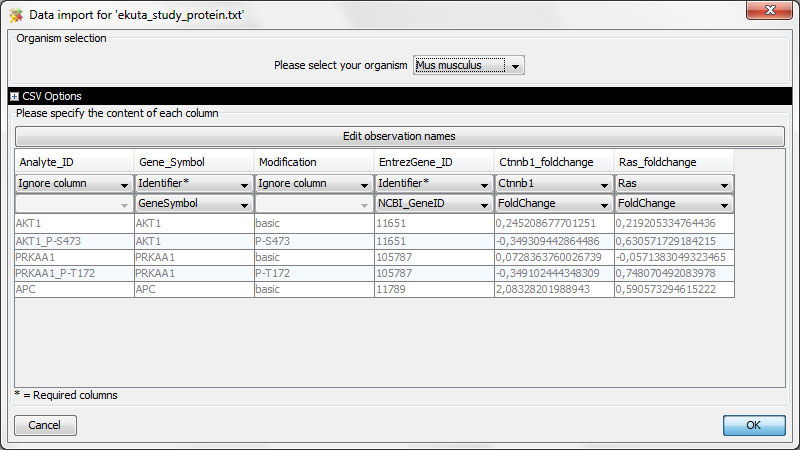
\includegraphics[width=1.0\columnwidth]{figures/import_dialog.jpg}}
\caption{
Example of the data import dialog. On the top, the species must be selected. The "CSV Options" panel might be expanded to correct auto-detected input file properties. At the table in the lower half, the content of each column must be specified. By clicking on the "Edit observation names" button, on can rename "Observation 1" to "Ctnnb1", as we did to create this example picture.
}\label{fig:inputdialog}
\end{figure}

In general, all data must be processed expression data in tabular text files (see Section~\ref{ch:prepare} for descriptions and examples of the input file formats). Then, there are many possibilities to open datasets in InCroMAP. For example, you can simply drag\&drop data into the application or select "File", "Open" to open a file. In the upcoming dialogs, you will need to define which type of microarray data is contained (mRNA, miRNA, DNA methylation or protein) and which columns contain what information.

Figure~\ref{fig:inputdialog} shows an example of the file input dialog. First, the species must be selected (on top of the dialog). If the input file format has not been inferred automatically, one may click on the black "CSV Options" label to specify further options (like "column separator char" or if the file contains headers - see Figure~\ref{fig:csvoptions}).


\begin{figure}[h]
\centerline{\noindent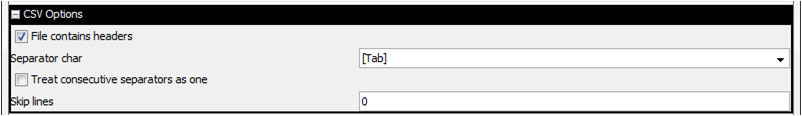
\includegraphics[width=1.0\columnwidth]{figures/expanded_csv_options.jpg}}
\caption{
Expanded "CSV Options" allow to give details for the input file. These properties are auto-detected and only need to be changed if the auto-detection failed to correctly infer those properties.
}\label{fig:csvoptions}
\end{figure}

In the table at the lower half of this dialog, one must specify the content of each column. This can be done by clicking on the combo box below the captions. In some cases (e.g., when selecting "Identifier"), another combo box below the first one will become available and the content must be further specified (e.g., when selecting "Identifier", this can be either a "Entrez Gene ID", "Gene Symbol", "Ensembl Gene ID", etc. - see Figure~\ref{fig:assigngeneid} for an example).

\begin{figure}[p]
\centerline{\noindent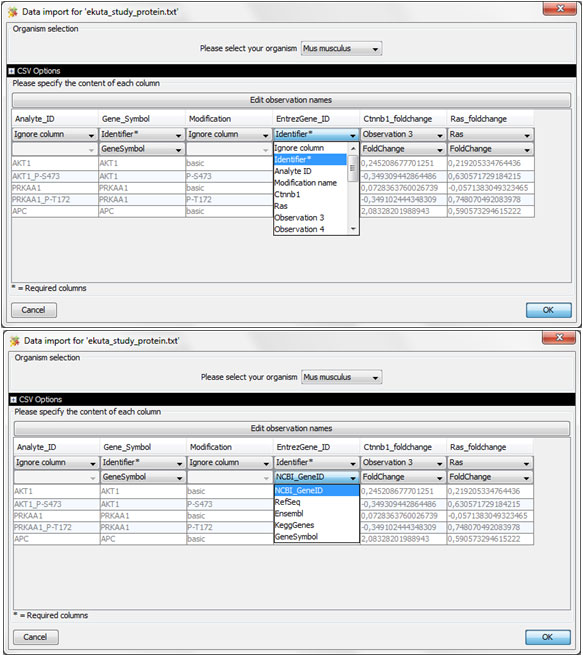
\includegraphics[width=1.0\columnwidth]{figures/assign_geneid.jpg}}
\caption{
Example for specifying column contents. In this example, Entrez Gene IDs are given as the content of one column.
}\label{fig:assigngeneid}
\end{figure}

\subsection{Importing observations from expression data}

Section~\ref{ch:prepare} gives examples for input files and specifies, what columns are required for each data type. Besides the data type specific columns, each dataset must have columns, containing your expression data as processed observations. Currently, these can be fold-changes or p-values. To import the fold-changes or p-values, an observation must be assigned to a column by picking "Observation \{Number\}" from the content combo box. Then, another combo-box will become available, which let's the user choose if the content contains fold-changes or p-values. This step is demonstrated in Figure~\ref{fig:importobservations} and must be performed for all observations one might want to import. The term "Observation" here refers to any column that contains experimental results as fold-changes or p-values.

\begin{figure}[!h]
\centerline{\noindent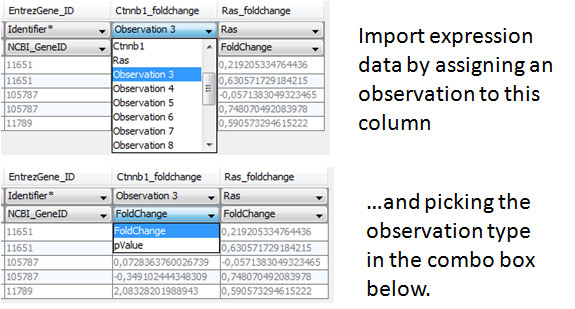
\includegraphics[width=.8\columnwidth]{figures/import_observations.jpg}}
\caption{
Importing processed observations from expression data into the application.
}\label{fig:importobservations}
\end{figure}

\subsection{Renaming observations}

The name "Observation" might be very unspecific for many datasets. Therefore, above the table on the import dialog is a big button "Edit observation names". This button allows renaming all "Observations" to, e.g., "DMSO\_vs\_KO" or any other more meaningful name. If the input file contained column headers and all observations are already assigned to columns on the input file dialog, InCroMAP will automatically suggest taking the column headers as observation names, as soon as the button "Edit observation names" is pressed. Figure~\ref{fig:renameobservations} demonstrates how to rename observations.

\begin{figure}[h]
\centerline{\noindent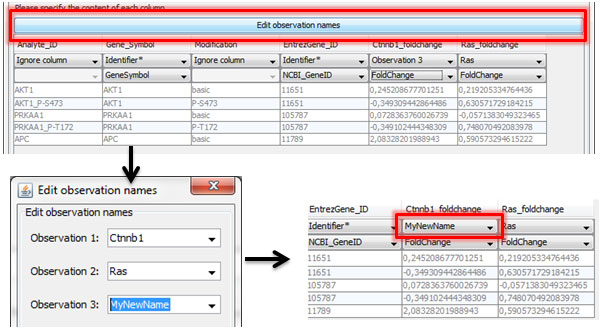
\includegraphics[width=1.0\columnwidth]{figures/renaming_observations.jpg}}
\caption{
To rename observations, click the large "Edit observation names" button. In the upcoming dialog, you may enter new names for each observation. The new name will become effective immediately.
}\label{fig:renameobservations}
\end{figure}










\chapter{Single dataset analysis examples}
This section describes some brief examples how to get started with single dataset analysis in InCroMAP.
As soon as you imported your data into the application, you'll see a table in a new tab, showing your data. On top of the tabs is a toolbar, showing some analysis functions. This toolbar always changes, depending on what is shown in the currently selected tab.

\section{Enrichment analysis (every platform)}
\label{sec:enrichment}
There are two ways to perform an enrichment analysis. One is to manually select lines in the table (corresponding to probes or genes) and right click on one of the selected lines. Then you can select an enrichment method (e.g., Gene Ontology or KEGG pathway) to perform this analysis.

The other way is to click the enrichment button in the Toolbar. Then, one needs to select an enrichment type to define a filter to select probes/genes for an enrichment. For example, one can pick a fold-change column, select "$\mid>=\mid$" (which is the same as "$\geq\pm$") and enter $1.0$ in the last field. This would lead to an enrichment on all genes that are differentially expressed with a fold-change cutoff of $1.0$ (i.e. "$fold-change\geq\pm1.0$").

\section{Pathway-based microarray data visualization (every platform)}
\label{sec:visualizeanydatainpathway}
InCroMAP offers multiple possibilities to visualize expression data in a pathway plot. One is, to select the tab containing the table with the input dataset and click on the "Visualize in pathway" button in the toolbar. In the upcoming dialog, one needs to pick the pathway of interest and an observation that contains the microarray data that should be visualized in the pathway. This will result in a picture, similar to Figure~\ref{fig:mapkmrna}.

\begin{figure}[htb]
\centerline{\noindent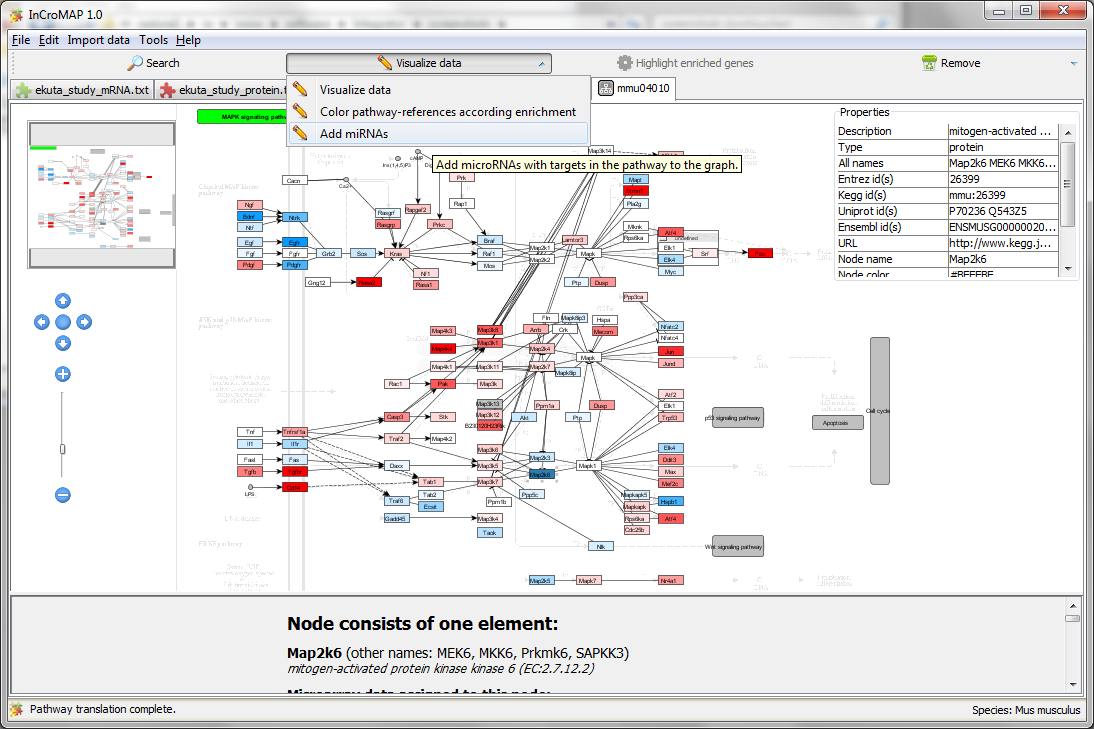
\includegraphics[width=1.0\columnwidth]{figures/9.png}}
\caption{
Example of the "MAPK signaling pathway" with visualized mRNA fold-changes (encoded as node-colors). The "Map2k6" gene-node has been selected and the bottom shows a detail panel, containing detailed information about this gene and all associated expression data.
}\label{fig:mapkmrna}
\end{figure}

Another possibility is to somehow visualize a pathway (e.g., directly from a pathway enrichment analysis or by selecting "Import data" and "Show pathway" from the menu bar) and then click "Visualize data" and again "Visualize data" from the toolbar. See the top of Figure~\ref{fig:mapkmrna} for a screenshot of this option. Then, one needs to select the dataset that should be visualized in the pathway and the observation within this dataset. After clicking "Ok", the data will be visualized in the pathway.

\section{Show microRNA targets (miRNA only)}
\label{sec:showmirnatargets}
When a tab with microRNA data is currently visible, one can select "Targets" and "Annotate targets" from the toolbar. Then, in the upcoming dialog, one can choose which databases should be used to annotate micro RNA targets. There are currently three experimentally derived target databases (miRecords \citep[see][]{miRecords}, miRTarBase \citep[see][]{miRTarBase} and TarBase \citep[see][]{TarBase}) and three databases with predictions (ElMMo \citep[see][]{ElMMo}, DIANA-microT \citep[see][]{DIANA} and TargetScan \citep[see][]{Targetscan}) available.

Please note that for all predictions only targets that are above the suggested "high-confidence" threshold of the corresponding prediction database have been included in InCroMAP. Targets with low or medium prediction confidence have not been included at all.

Furthermore, many researchers follow the rule that "the more prediction methods suggest a target, the more reliable is this information". This rule has not been implemented into InCroMAP, because it is controversial. There are multiple reviews, suggesting that it is better to use one good prediction algorithm, than combining multiples with an "AND". The three prediction methods offered by InCroMAP have been proven to be good prediction methods and also to perform good in combination. See \cite{Alexiou2009} for a verification of these statements and further information on micro RNA targets.

\section{Visualize microRNA targets (every platform)}
When a tab, containing a pathway plot (as shown, e.g., in Figure~\ref{fig:mapkmrna}) is currently selected, users can click "Visualize data" and "Add miRNAs" to visualize micro RNAs as small rectangles with edges to their mRNA targets. This can be done, even if no miRNA expression data if available. For more information on the upcoming miRNA target database selection dialog, see Section~\ref{sec:showmirnatargets}.


\section{Genome region plot (DNA methylation only)}
\label{sec:dnamxyplot}

\begin{figure}[htb]
\centerline{\noindent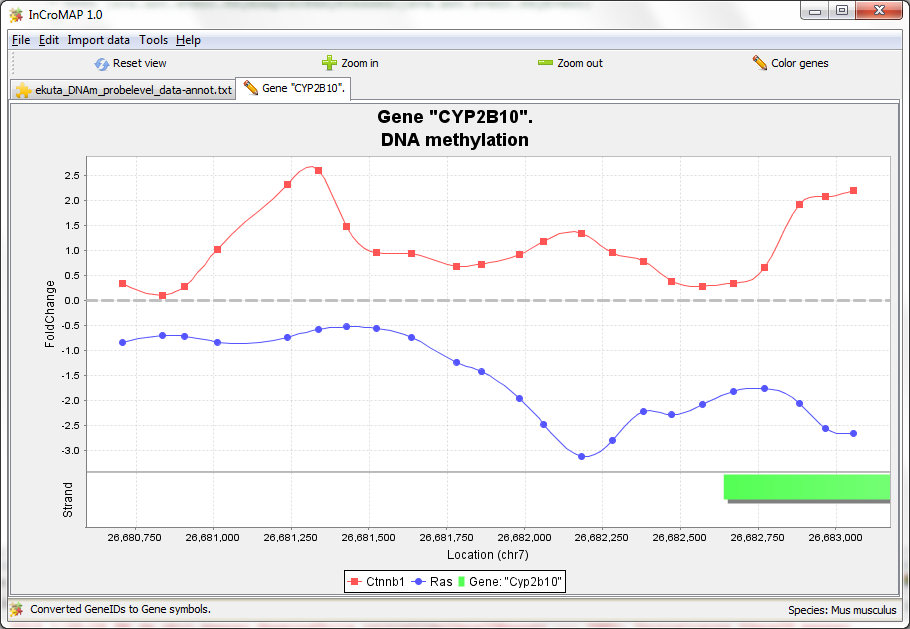
\includegraphics[width=1.0\columnwidth]{figures/me.png}}
\caption{
XY-plot of DNA methylation data in the promoter region of the "Cyp2b10" gene.
}\label{fig:dnamplot}
\end{figure}

DNA methylation data can be visualized as genome-region XY-plot. Please select a tab, containing DNA methylation data. There are now two possibilities to generate such a plot: The quick method is by selecting a probe (i.e., a line in the table), make a right click on it and select "Plot genome region". The application will then collect all probes that are associated with the same gene and create a genome region plot of them (see Figure~\ref{fig:dnamplot} for an example).

The other possibility is, to click the "Plot genome region" button in the toolbar. The upcoming dialog then let's you pick either a custom region by manually specifying chromosome, start and end coordinates. Or, after clicking "Plot a region, associated with a gene", you can select any gene and let InCroMAP plot all probes that are associated with this gene.
At the bottom of this dialog, you can pick an observation from the current dataset that should be plotted. To include multiple observations in one plot (e.g., Figure~\ref{fig:dnamplot} has two observations called "Ctnnb1" and "Ras"), one can pick "Include other observations with same signal type" (signal type refers to either p-values or fold-changes). If "Do not include other observations" is selected, only the selected observation will be plotted.


\section{Metabolic overview (mRNA only)}

Creating metabolic overviews is a good way to get started with novel mRNA expression datasets. This will create a plot that is similar to Figure~\ref{fig:metabolicpathways}. As this is an advanced analysis example, please make yourself familiar with the application before trying to follow the described steps.

\begin{figure}[htb]
\centerline{\noindent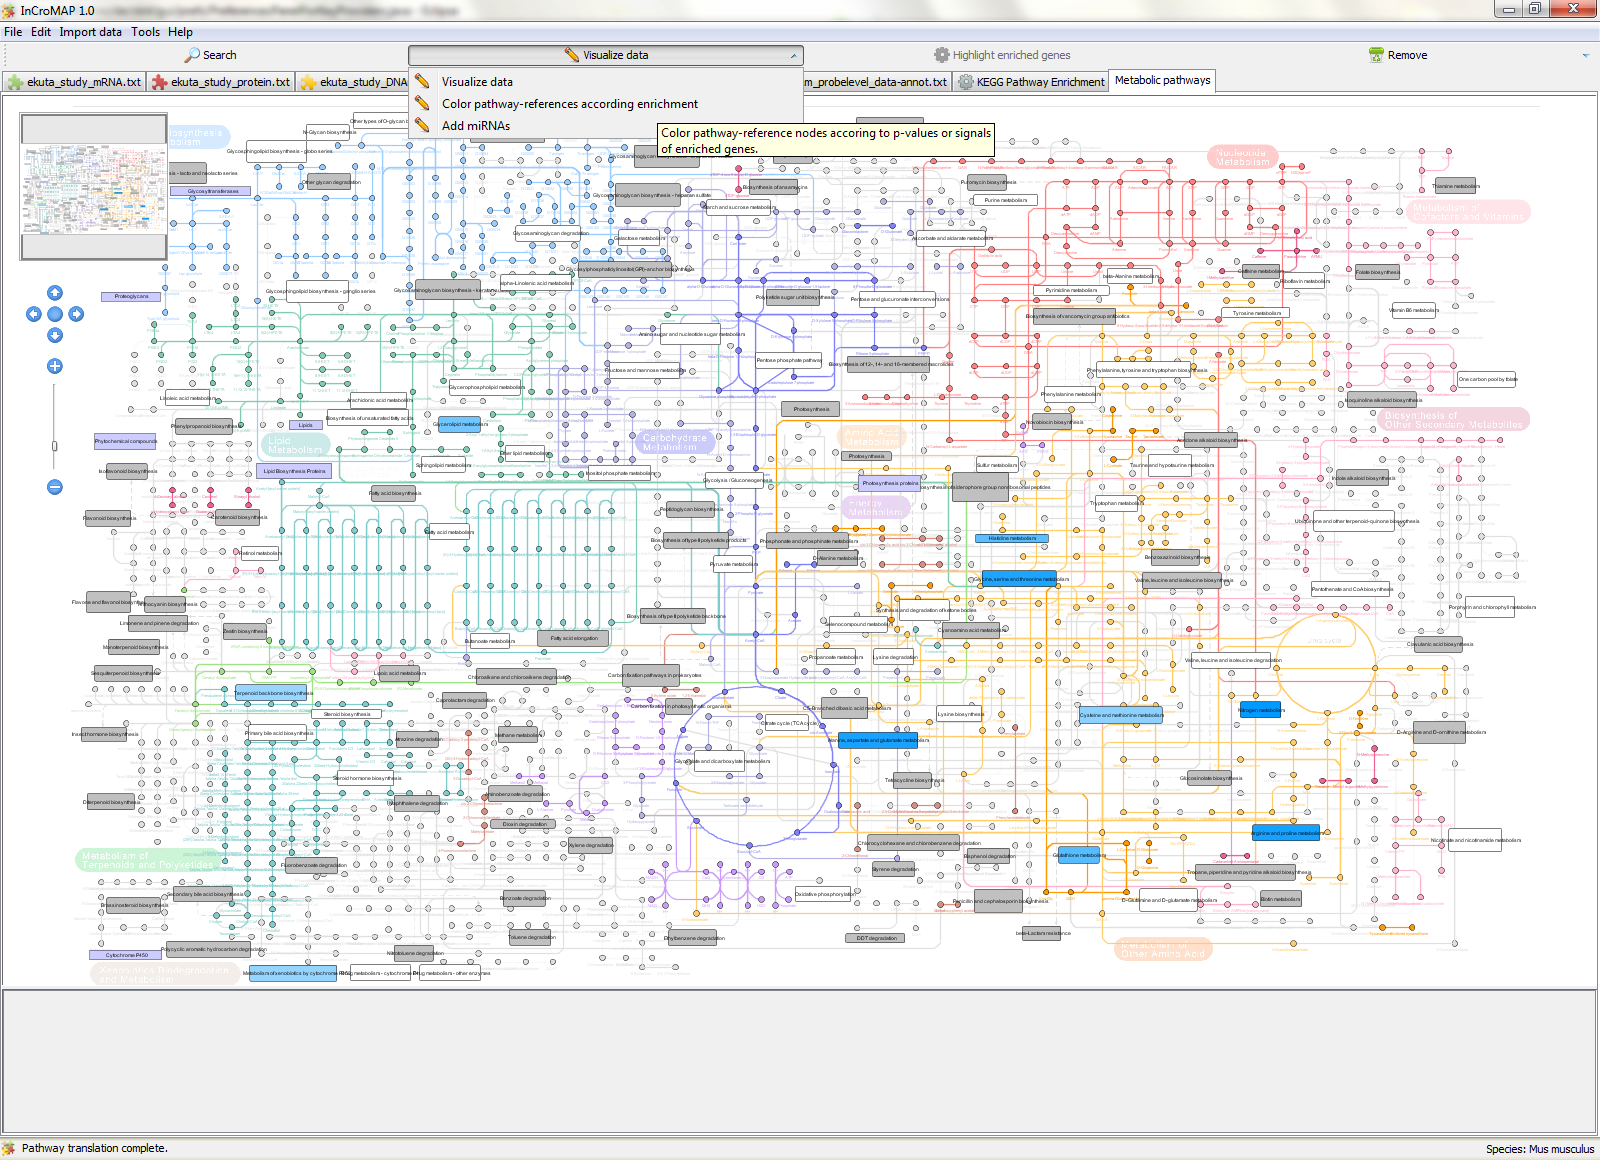
\includegraphics[width=1.0\columnwidth]{figures/mp.png}}
\caption{
InCroMAP visualization of a metabolic overview pathway. All other referenced pathways (rectangle shaped nodes) are colored according to their enrichment p-value (i.e., how significant they are altered in input dataset). The darker-blue they are, the lower the p-value. White means $p-value\geq0.05$ and grey means, that this pathway is not altered at all (not contained in pathway enrichment).
}\label{fig:metabolicpathways}
\end{figure}

From the application, select a tab that contains mRNA data. From this tab, select "Visualize in pathway". In the upcoming dialog pick "Metabolic pathways" from the pathway-selection combo-box and any observation of interest from the combo-box below the pathway selection. After clicking "Ok", the application might need some time to fetch all required data from the KEGG-API.
The result will now be a pathway, similar to Figure~\ref{fig:metabolicpathways}, in which all edges correspond to the mRNA expression level of enzymes. I.e., the colored edges express the mRNA fold-change (or p-value, depending on the selected observation) of the appropriate enzyme. You can click on a colored edge to get more information. Please note that in other pathways the mRNA expression levels are visualized as colored rectangles, whereas in the "Metabolic pathways"-pathway all mRNA expression levels are encoded in colored edges!

In this overview-pathway, it is also possible to visualize the importance of specific metabolic pathways. Please go back to your mRNA data tab and perform a KEGG pathway enrichment, as described, e.g., in Section~\ref{sec:enrichment}. Now go back to the metabolic overview pathway again and select "Visualize data" and "Color pathway-references according enrichment" from the toolbar. Select the just performed KEGG pathway enrichment result in the appearing dialog and click "Ok". All nodes that are to references to other pathways (big rounded rectangles) now get colored according to the p-value in the selected pathway enrichment. I.e., the deeper blue they are, the more significant is the pathway (and the enrichment p-value). A white color is assigned to not significantly enriched pathways and grey means, that this pathway is not altered at all (did not appear in the enrichment). Figure~\ref{fig:metabolicpathways} shows an example of the enrichment-based visualization of pathway-reference nodes.




\chapter{Integrated cross-platform microarray data analysis examples}

This chapter describes analysis methods in the InCroMAP application that are available to users who have data from two or more different platforms for the same samples.

\section{Integrated pathway-based visualization}

\begin{figure}[htb]
\centerline{\noindent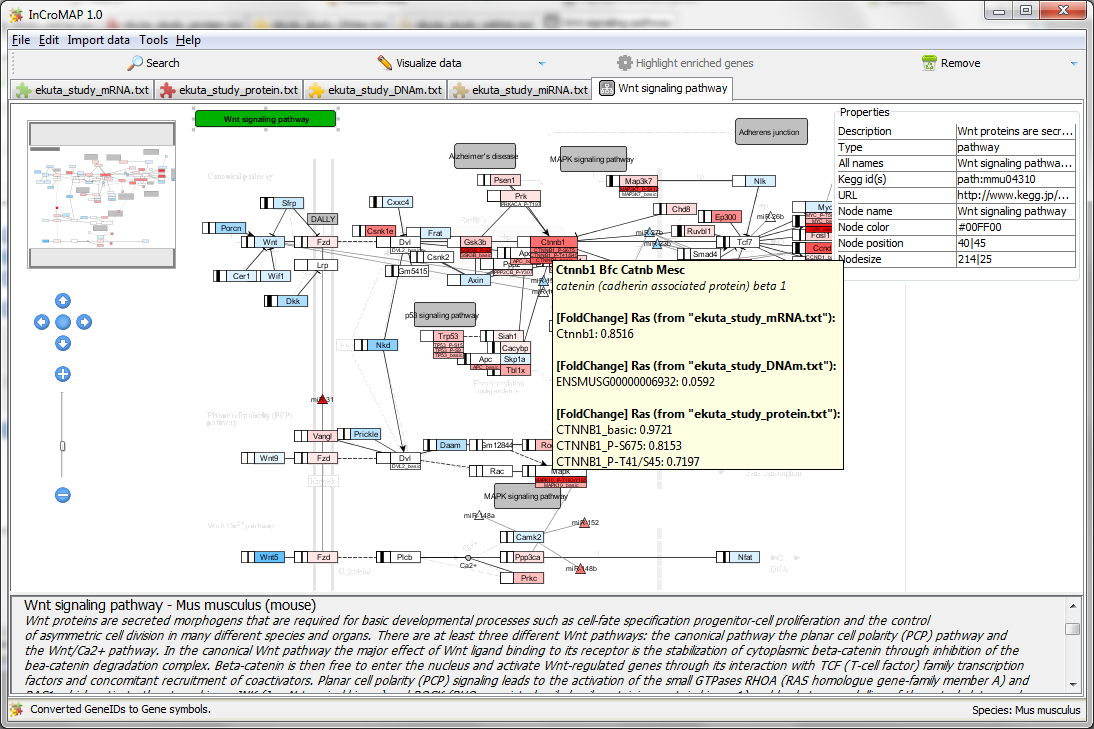
\includegraphics[width=1.0\columnwidth]{figures/10.png}}
\caption{
Pathway-based integrated cross-platform microarray visualization. This example shows the "Wnt signaling pathway". The rectangular nodes correspond to genes or gene families and their color indicates mRNA expression (blue means downregulated, red means upregulated). The box left of those nodes indicates promoter DNA methylation. The largest peak is shown and an empty box indicates no differential methylation. A bar to the left indicates hypomethylation and a bar, which goes from the middle of the box to the right indicates hypermethylation. Small rectangular boxes below the mRNA nodes indicate protein and protein modification expression. E.g., the "CTNNB1" gene has associated data from two different phosphorylation sites and the basic protein expression. Every of those boxes is red, which indicates upregulation. MicroRNAs are visualized as triangles with edges to their mRNA targets. MiRNA node color indicates miRNA expression.
}\label{fig:integratedWNTpw}
\end{figure}

Integrated pathway-based visualizations allow to visualize DNA methylation, mRNA expression, micro RNA expression and protein (modification) expression datasets in one pathway. See Figure~\ref{fig:integratedWNTpw} for an example. There are multiple ways to create such a visualization. You could just open any pathway and then visualize each of the datasets therein (see Section~\ref{sec:visualizeanydatainpathway}). Another easy way is to select "Tools" and "Integrated heterogeneous data visualization" from the menu bar. In the upcoming dialog, you first need to select the organism and the pathway of interest. For each data type is a checkbox in this dialog called, e.g., "Visualize mRNA data". Select the desired checkboxes and select a dataset and observation for each dataset (you need to have all datasets imported into InCroMAP, see Section~\ref{sec:opendata}). After clicking "Ok", a new tab with the pathway-based visualization of all your selected microarray datasets will show up.


\section{Data pairing}

\begin{figure}[htbp]
\centerline{\noindent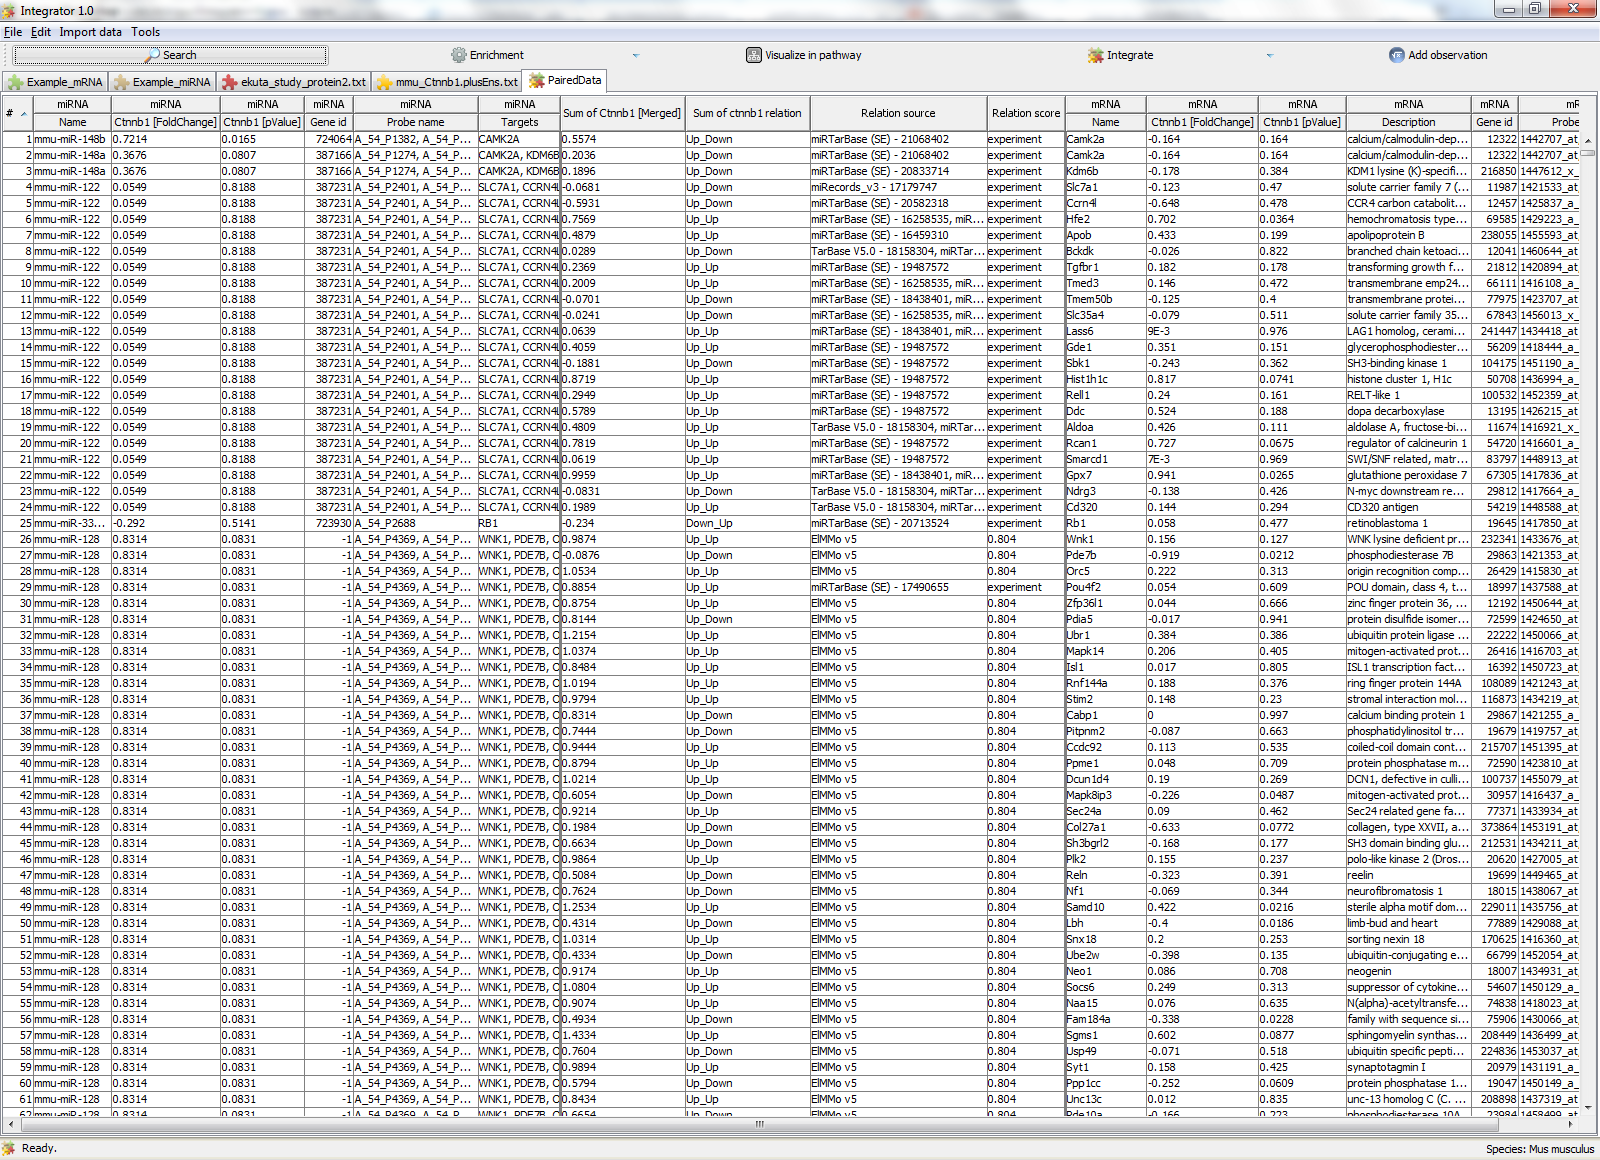
\includegraphics[width=1.0\columnwidth]{figures/e2.png}}
\caption{
Example of the cross-platform "Data pairing" analysis method. Here: an integrated mRNA and microRNA analysis. On the left part of the figure, a micro RNA dataset is shown with expression p-values and fold-changes for each miRNA. In the middle, the target relationship for each miRNA is shown (source database, eventually prediction score, etc.). On the right side, the matching mRNA target is shown together with p-value and fold-change. The "Up\_Down" column in the middle shows the relation of microRNA expression to mRNA expression (i.e., microRNA expression level is upregulated, mRNA expression level is downregulated).
}\label{fig:datapairing}
\end{figure}

Although this method makes especially sense for combinations with miRNA data, it can also be used for any other platform combination. Data pairing basically creates a huge table that puts one dataset in relation to another.
We are going to explain this on some mRNA and miRNA example datasets. The result will be an integrated mRNA and miRNA analysis table, that contains microRNA fold-changes, mRNA target relations, and corresponding mRNA fold-changes (see Figure~\ref{fig:datapairing}). Please select the tab, containing the tabular miRNA data. From the toolbar, select "Integrate" and "Pair data". In the upcoming dialog, you'll need to select the other dataset, which is in our example the mRNA dataset. Furthermore, you have the option to calculate a merged observation. This can be, e.g., the difference between miRNA and targeted mRNA expression fold-change or various other options. You can also unselect "Calculate a merged observation". After pressing "Ok", the paired table with two matched datasets will appear. If you haven't already annotated miRNA data with targets, the target database selection dialog (as described in Section~\ref{sec:showmirnatargets}) will show up before the final results.
The data pairing with micro RNA datasets will lead to three additional columns. One relation column that simplifies the miRNA expression fold-change and target fold-change relation. E.g., "Up\_Down" means that microRNA expression is upregulated and the target mRNA expression level is downregulated. The "Relation source" column gives the database(s), that contained or predicted this mRNA to be a target of the miRNA. In case of experimental databases, the PubMed identifier of the corresponding publication is given after the experimental database name. The third additional column is called "Score" and gives the score of the prediction method, if the target is a predicted target. Please refer to the corresponding miRNA target prediction databases itself for an interpretation of these scores. Please note that InCroMAP only shows targets that are above the recommended cutoff threshold for each miRNA target database. I.e., low confidence targets are not included in InCroMAP at all.

\section{Integrated enrichment}

Conventional enrichment analysis is just an interpretation of the current data type. For example, a pathway enrichment analysis on mRNA data will show pathways, that are altered in the mRNA dataset. Pathway enrichment analysis on DNA methylation data will show pathways that contain genes with significantly altered DNA methylation in their promoter regions.

With the integrated enrichment method in InCroMAP, the result of an enrichment analysis is not anymore just an interpretation of one platform - it's more close to what is really altered in the samples across multiple platforms. Therefore, the integrated enrichment is performed across multiple platforms and reflects alterations that occur on every (if datasets are connected with an AND) or any (if datasets are connected with an OR) platform.

To perform such an enrichment, please select "Tools" and "Integrated enrichment" from the menu bar. Now select your organism and all currently opened datasets from this organism should show up in the box below the organism selection. Pick all datasets that should be integrated into this enrichment (you can pick multiples by press and hold the CRTL-key of your keyboard) and select an enrichment type (Gene Ontology, KEGG pathway, etc.).
At the bottom of this dialog, you can select if all the probes/ genes from the datasets should get connected with an "AND" or "OR" operator. For example, if you choose "AND", every gene must be altered in all selected datasets to get selected for the enrichment analysis. We recommend selecting "OR", because, e.g., an alteration in DNA methylation must not always also show an alteration in mRNA expression.

After confirming this dialog with "Ok", a threshold must be given for each dataset to define which genes should be picked for the enrichment analysis. Once all thresholds are defined, the result of the enrichment will show up.

\section{Gene-based tabular integration of data from multiple platforms}

\begin{figure}[htbp]
\centerline{\noindent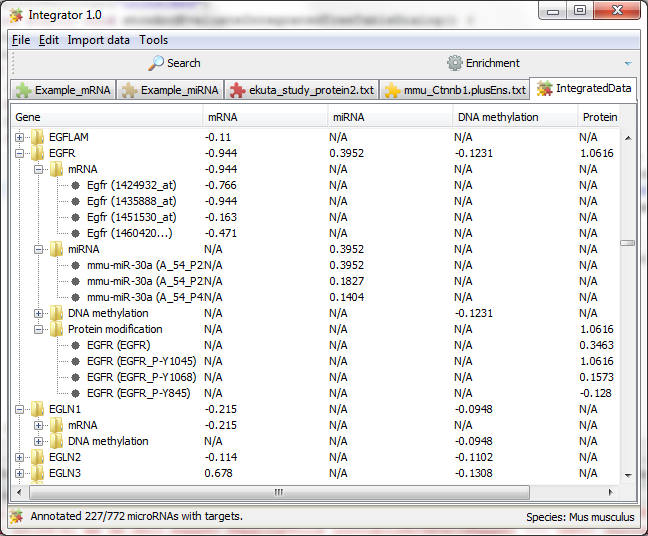
\includegraphics[width=1.0\columnwidth]{figures/7.png}}
\caption{
Example of an expandable, gene-based tabular view of microarray data from different platforms. Each top root node is one gene (e.g., the second row "EGFR") and each column shows the corresponding observation (in this example the fold-change) of each platform. If the node is expanded, novel nodes appear for each platform that contains data for this gene (e.g., the third row "mRNA"). If this is further expanded, the single values associated with this gene on the particular platform show up (in this example, all mRNA probes). For miRNA datasets, all miRNAs targeting this gene are shown.
}\label{fig:tabularintegration}
\end{figure}

Another method to get a cross-platform view of various samples is the expandable, gene-based tabular integration of heterogenous datasets. An example can be seen in Figure~\ref{fig:tabularintegration}. At the root level, each row corresponds to one gene. In the columns, the associated values of various platforms are denoted. If one gene is expanded, second-level nodes show up that are named according to the platform (e.g., "mRNA"). If these nodes are expanded, the single probes associated with this gene appear. Thus, this integration method gives a possibility to quickly examine expression data, coming from various different platforms if one already knows some genes of interest.

To create such a table, select "Tools" and "Integrate heterogeneous data" from the menu bar. In the upcoming dialog, please select your organism and set a checkmark on every platform you want to integrate. Then, pick a dataset and an observation for each platform. Please note that this is a gene-centric table. Thus, each dataset needs to be converted to contain gene-centric values. Therefore, you can select if you want to do this by calculating the mean, median, maximum, etc. in another combobox below the observation selection. You can pick separate options here for each platform. After confirming this dialog, the result table like shown, e.g., in Figure~\ref{fig:tabularintegration} will appear.



\chapter{Help for different tabs and methods}

\section{Tabular tabs in general - searching, sorting and more}

All input data from every platform is shown as a table. The first row is the header, which usually contains items like "\#" (which is a simple number counting from one to infinity for every row) or "Name". You can click on any of those column headers to sort the table according to this column.

All tables in InCroMAP can be searched, by simply clicking on any row in the table (i.e., setting the focus on the table) and start typing. This will result in a text field to show up at the top left corner of the table. The table selection will automatically change to select an object that contains what you searched for. If you want to search for the next element, containing the same string, you need to press "F3" on your keyboard. Pressing "F3" once more will again search for the next hit, etc.

\section{Enrichments and enrichment tabs}

\begin{figure}[htb]
\centerline{\noindent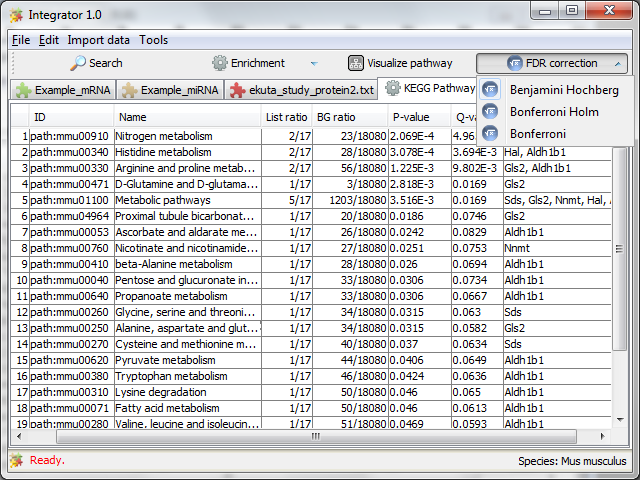
\includegraphics[width=1.0\columnwidth]{figures/6.png}}
\caption{
InCroMAP screenshot that shows the result of a KEGG pathway enrichment. The "FDR correction" menu shows different methods to face the problem of multiple testing.
}\label{fig:enrichmentExample}
\end{figure}

InCroMAP currently offers three different enrichments: KEGG pathway, Gene Ontology, and any enrichment using MSigDB files. For the first two, all required data will be obtained automatically. You just need to select genes for the enrichment (e.g., by setting a threshold for the fold-changes or p-values). The MSigDB enrichment will require you to specify a gene set file. You can download any gene set in GMT format from the molecular signatures database (MSigDB) at \url{http://www.broadinstitute.org/gsea/msigdb/} (see \cite{MSigDB}). On this homepage, please either download the "gene symbols" files or make sure that the "entrez genes ids" from the other files are valid for your current organism! For example, you can't perform an enrichment on a mouse dataset if the MSigDB file contains entrez gene ids for human. If you select "MSigDB enrichment" from within InCroMAP, the application will ask you to specify a path to any file, containing a gene set from the molecular signatures database as mentioned above.



\subsection{How is the enrichment performed? And what are the columns?}
\label{sec:enrichmenthowto}

InCroMAP first creates a gene-pool and then calculates p-values for every pre-defined gene set (e.g., pathway or GO-term) for this gene-pool. The results are presented to the user in a new table. The mentioned gene-pool is created by the user, typically by picking all significant genes ($p-value<0.05$ or $abs(fold-change)>1.5$). The gene sets are predefined by KEGG, Gene Ontology or the MSigDB. Now for every gene set, we investigate if it contains one or more genes from our gene-pool. The result is denoted in the "List ratio" column. This column denotes the number of genes from our gene-pool list that are in the gene set, described by the row, and the total gene-pool size. The "BG ratio" column denotes the total number of genes in the gene set and the total number of all genes in any gene set. From these values, the raw "p-value" is calculated using a hypergeometric test. The "q-value" column contains p-values, that have been corrected for multiple testing. By default, all p-values are being corrected using the "Benjamini \& Hochberg" FDR correction method (see \cite{BenjaminiHochberg}). This can be changed to "Bonferroni" or "Bonferroni Holm" by clicking on the "FDR correction" button in the toolbar (see Figure~\ref{fig:enrichmentExample}). The last column denotes the actual genes from the gene-pool that are in the current gene set.

\textbf{Example:} we have created a KEGG pathway enrichment with some p-value cutoff on an mRNA dataset. After applying the threshold, we had a total of 17 genes in our gene-pool. The results of the enrichment are depicted in Figure~\ref{fig:enrichmentExample}. The third row now denotes an enriched pathway (i.e., gene set) called "Arginine and proline metabolism". Two of our 17 genes in the gene-pool are contained in this pathway. The pathway has a total of 56 genes and the total number of genes occurring in any pathway is 18080. From these values, the p-value of 0.001225 is calculated with a hypergeometric test and, using Benjamini \& Hochberg, the corrected p-value is 0.009802. The two genes from our gene-pool that are in the pathway are "Gls2" and "Aldh1b1", what is denoted in the last column.

\textbf{For micro RNA datasets}, the enrichment is a little bit more difficult. The gene sets behind these enrichment are mostly referring to protein coding genes. Thus, they are not directly usable for micro RNAs. Hence, the enrichment on miRNA datasets is performed on the targets of the corresponding miRNAs. So first, you need to annotate your miRNA dataset with targets, using the "Targets" and "Annotate targets" button on the toolbar. Then, as with every other dataset you can define a threshold for the p-values or fold-changes. This will result in a microRNA pool that meets the selected cutoff. This microRNA pool is now converted to a gene-pool by using all annotated targets from the microRNAs in the pool. The rest of the enrichment is the same procedure as described above. Except for the list ratio, which denotes the number of microRNAs that contain targets in this gene set (i.e., pathway) and the total number of microRNAs in the gene pool. In the preferences, you can change the list ratio when performing a microRNA enrichment to reflect the number of targets in this gene set, instead of the number of microRNAs that contain targets in the gene set.


\section{Pathways and the pathway visualization tabs}

The InCroMAP pathways are graphs that are layouted on top of an original KEGG pathway picture. In general, small circular nodes are small molecules, rectangular nodes with rounded corners describe referenced pathways (also called "pathway-reference nodes"), and rectangular-shaped nodes (smaller ones, without rounded corners) correspond to products of genes or gene families. Please note that KEGG sometimes puts multiple genes into a single node and if it's easier to visualize, a node can have multiple instances in a graph. Sometimes (e.g., in the "Metabolic pathways"-pathway), the proteins or enzymes are shown as big edges, connecting compounds. These are rare special cases that KEGG uses to enhance the quality of the overall picture. In these cases, only mRNA data can be visualized (resulting in a color-change of this big edge).

In every pathway, you can double click on a pathway-reference node to open the corresponding pathway in InCroMAP or you can click on any other node or edge to get further information about it. Furthermore, you can search for certain genes or other strings in a pathway, by selecting "Search" from the toolbar. This will change the font and border color of all nodes matching your search to red.

\subsection{Visualize expression data in a pathway}
\label{sec:visdatainpw}
When a pathway tab is currently visible, any opened expression dataset can be visualized in the pathway by selecting "Visualize data" and again "Visualize data" from the toolbar. Only one dataset per type (i.e., mRNA, miRNA, protein, or DNA methylation) can be visualized at a time, but all types can be visualized at once. In the following part we are referring to the default properties. Many options (like the color or threshold for upregulation) can be changed in the preferences!

\begin{figure}[htb]
\centerline{\noindent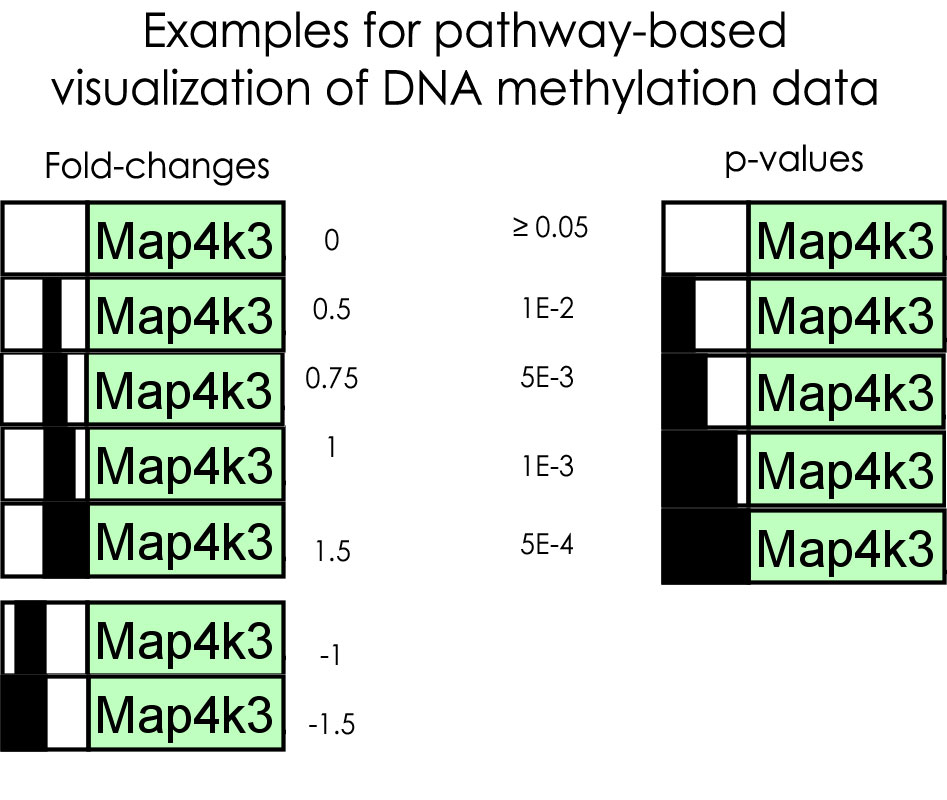
\includegraphics[width=0.6\columnwidth]{figures/pw-dnam.jpg}}
\caption{
Examples of various fold-changes or p-values for DNA methylation data and their visualization in InCroMAP. These examples are only valid for the default settings. For example, the p-value required to fill the whole box can be changed in the preferences. Usually, the value visualized for a gene corresponds to the maximum peak in the gene promoter - but this can also be changed in the preferences.
}\label{fig:dnampw}
\end{figure}

For all data types, except DNA methylation, if fold-changes are visualized, the color red means upregulation and blue means downregulation. The darker the color, the higher/lower is the fold-change. Default requirement for a node to get the darkest red/blue color is a fold-change of $\pm1.5$. White color indicates no differential expression (by default, fold-changes between $\pm0.5$) and grey color means, that no value from the input dataset could be linked to this node (e.g., gene was not on microarray, removed by preprocessing, etc.). These properties are similar when visualizing p-values. A white color, by default, means that the p-value is $> 0.05$ and grey means, that no data is available. Significance is indicated by the darkness of the blue color on a log-scale, where $0.0005$ is the threshold for the darkest blue color. All these properties (thresholds, colors, etc.) can be changed in the preferences.

To visualize data in a pathway, only one value for a node in the pathway can be visualized. These "nodes" are mostly genes, but sometimes also gene families (e.g., in the "MAPK signaling pathway", "MAPK1" and "MAPK3" are summarized in one node). Thus, InCroMAP sometimes needs to merge multiple probes and values to a single value. In the preferences, you might want to remove the checkmark on the "Remember gene center decision" box. If this is unchecked, InCroMAP will ask every time how the input data should be gene-centered. Therefore, several options are available: Mean, Median, Minimum, Maximum, Maximum distance to zero (i.e., $\max{|x|}$), NormalizedSumOfLog2Values, or Automatic. Automatic will take the most significantly probe (p-values) or the probe with maximum differential expression (fold-changes). Please see the chapter "\nameref{chp:preferences}" for more information on these options.

\begin{figure}[htb]
\centerline{\noindent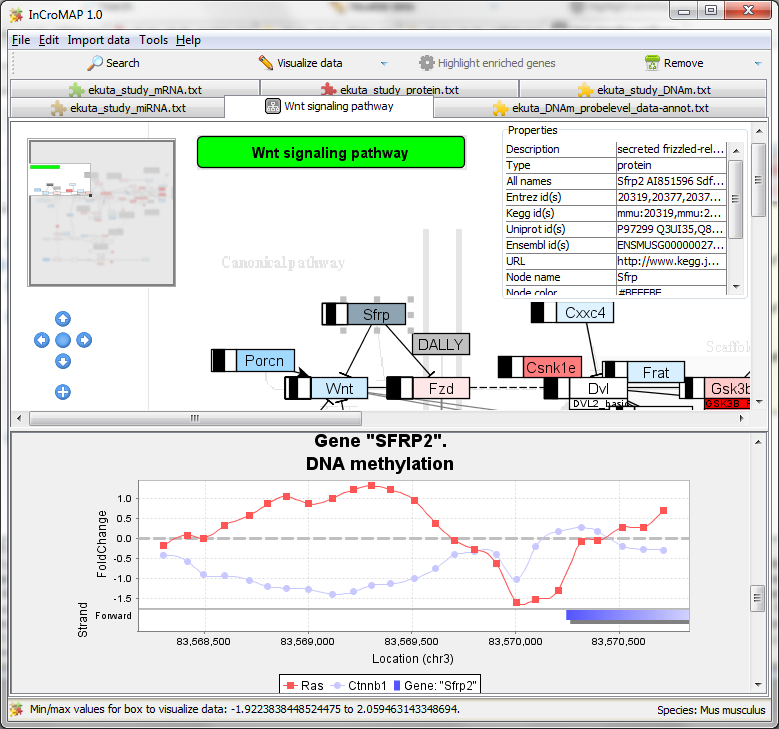
\includegraphics[width=0.8\columnwidth]{figures/1-1.png}}
\caption{
Example of an integrated pathway-based visualization. Here, three different data types (mRNA, protein and DNA methylation) have been visualized. The node "SFRP" is selected and the bottom half shows a detailed view of all expression data associated with this node. The DNA methylation data is plotted in detail as genome region plot of this gene.
}\label{fig:integratedpwdnamdetails}
\end{figure}

Messenger RNA is visualized by changing the color of the rectangle-shaped nodes, according to mRNA expression. MicroRNA is visualized, by changing the color of the triangle-shaped miRNA nodes, according to miRNA expression. Protein data is visualized, by adding small boxes below the rectangle-shaped nodes. DNA methylation data is visualized, by putting black boxes left of the rectangle-shaped nodes. For DNA methylation, the same thresholds as for all other data types are valid. But the expression is not encoded in a color, but in a black bar that goes from the middle to the left, if the gene is hypomethylated and to the right, if the gene is hypermethylated. For p-values, a black bar goes from the left border of this box to the right one, depending on the significance. See Figure~\ref{fig:dnampw} for examples and more details on the pathway-based visualization of DNA methylation data. With the default settings, the probe with maximum differential expression or maximum significance in the promoter determines the value for DNA methylation visualization of this gene. This is very similar to maximum peak detection approaches! But still, DNA methylation data is not very informative if it is summarized to a single value per gene and thus, InCroMAP includes a detail panel that contains a plot of the DNA methylation data in the genomic and promoter region of the selected gene. The black bar, added to the pathway, should show in a very simplified view which genes are interesting and important. For those genes then, the user can click on their nodes and in the lower half of the application a new frame is shown with detailed information about the nodes and all expression values associated with them. Please see Figure~\ref{fig:integratedpwdnamdetails} for an example of the detailed DNA methylation visualization.


\subsection{Other pathway-based visualization options}

If you started by performing a KEGG pathway enrichment on your expression data and then selected a pathway from the enrichment and clicked "Visualize pathway", then the "Highlight enriched genes" option will become available in the toolbar. If this option is selected, each node in the pathway is colored grey, except for nodes that correspond to genes that were enriched in this pathway. These are highlighted in yellow (which is only a highlighting and does not express up- or downregulation). For example, Figure~\ref{fig:enrichmentExample} shows the result of an enrichment. If we would select the third row ("Arginine and proline metabolism") and click on "Visualize pathway", then the "GLS2" and "ALDH1B1" genes would be highlighted in yellow.

Another visualization possibility (when a KEGG pathway enrichment has been performed) is coloring pathway-reference nodes according to the enrichment p-value. This can be done by selecting "Visualize data" and "Color pathway-references according enrichment" from the toolbar. This will change the color of all pathway-reference nodes (rectangular nodes with rounded corners) according to their p-value in the enrichment. The color scheme and requirements are the same as described in Section~\ref{sec:visdatainpw}. An example of such colored reference nodes can be seen in Figure~\ref{fig:metabolicpathways}.



\section{DNA methylation plots}

InCroMAP can create genome-region, XY-plots of DNA methylation data. The DNA methylation data is plotted on the upper part of the figure and all genes in this genome region on the bottom. See Figure~\ref{fig:dnamplot} for an example. Section~\ref{sec:dnamxyplot} describes in detail how to create such a plot and how to select which observations should be contained in the plot.

\noindent \emph{Hint: To get the full name of a depicted gene, you can hover the gene with your mouse cursor and a tooltip with the full gene name will appear.}

\subsection{Integrated mRNA expression and DNA methylation plots}

When a tab, containing only the XY-plot of DNA methylation data, is selected, InCroMAP can change the color of the genes at the bottom of this graph according to another expression dataset. Therefore, you can click on the "Color genes" button in the toolbar and select an expression dataset. This is very similar to changing the color of the pathway nodes. For example, you can create a DNA methylation plot of a custom genome region and select "Color genes" from the toolbar. Then, you have to select the dataset and observation you wish to use for coloring the gene (e.g., an mRNA dataset). InCroMAP will then change the color of all the genes, depicted at the bottom of this graph, according to the selected dataset. The colors and thresholds for this procedure are the same as for the pathway-visualization (see Section~\ref{sec:visdatainpw}).



\chapter{Preferences}
\label{chp:preferences}

There are many preferences that you can change to influence the analysis results and generic behavior of InCroMAP. Please note that any changes made to the preferences are only valid for new tabs/ analyses. E.g., if you add a navigation panel to the pathway tabs, it will not show up on the existing, but on all novel tabs.


\section*{InCroMAP options}
These options influence generic InCroMAP properties, like how to merge multiple probes or how to visualize data in a pathway.
\begin{description}
  \item[Gene center signals by] For many operations, all signals (i.e., observations, fold-changes, etc.) that belong to one or multiple genes must be summarized to one value. For example, when visualizing data in a pathway, one value must be calculated that corresponds to one node. The following options are available for this calculation: Mean, Median, Minimum, Maximum, Maximum distance to zero (i.e., $\max{|x|}$), NormalizedSumOfLog2Values (i.e., $\frac{\sum\limits_{i=1}^n\log_2 x}{n}$, useful for p-values), or Automatic. Automatic will take the minimum for p-values, "maximum distance to zero" for fold-changes, and mean for all others. This corresponds to taking the most significant probe (p-values) or the probe with maximum differential expression (fold-changes).


  \item[Remember gene center decision] If this is unchecked, InCroMAP will ask every time how to merge multiple signals (i.e., the "Gene center signals by" option). If it is checked, the current value will be taken as default value without asking each time.

  \item[Count miRNA targets for list ratio] InCroMAP requires protein coding genes for enrichments. Hence, for miRNA datasets, InCroMAP will take the miRNA targets of the selected miRNAs to  perform the enrichment. The p-value of the enrichment depends on the list ratio (all terms explained in detail in Section~\ref{sec:enrichmenthowto}). By default, InCroMAP will take the number of microRNAs that have targets in the current pathway and the total number of microRNAs in the gene-pool as list ratio. By selecting this option, InCroMAP will count the number of targets to calculate the list ratio, rather than the microRNAs themselves. I.e., number of targets of any microRNA from the gene-pool that occur in the current pathway and total number of all targets from all microRNAs in the gene-pool.

  \item[Fold change for maximum color] This is the fold-change that is required for a gene to get the color that is defined some options below. All fold-changes closer to zero get brighter colors assigned.
  \item[Don't visualize fold changes between $\pm$ x] All fold-changes between $\pm$ this value will get the "Color for no fold change".
  \item[P-value threshold for maximum color] This is the p-value that is required to get the full "Color for minimum fold change" assigned. All greater p-values will get brighter colors.
  \item[Don't visualize p-values $>$ x] All p-values greater than this value will get the "Color for no fold change".
  \item[Color for X] Define various colors (the "Color for no value" is assigned to all nodes that can not be mapped on your input dataset).

  \item[DNA methylation maximum box width] Define the width of the black boxes (in pixels) that appear when visualizing DNA methylation data in a pathway.
  \item[Protein modification box height] Define the height of the boxes (in pixels) that appear below the nodes when visualizing protein data in a pathway.
\end{description}



\section*{KEGGtranslator options}
These options influence the creation of the pathways from the source database.
\begin{description}
  \item[Remove orphans] If true, remove all nodes that have no edges before translating the pathway.
  \item[Label genes by] For one KEGG object, multiple names are available. Choose how to assign one name to this object.
  \item[Show formula for compounds] If true, shows the chemical formula for all compounds, instead of the name.
  \item[Remove white gene nodes] If true, removes all white gene-nodes in the KEGG document. KEGG usually draws all enzymes that occur in homologous, but NOT the current organism in white.
  \item[Remove pathway references] If true, removes all pathway-reference nodes.

  \item[Merge nodes with same edges] If true, merges all nodes that have exactly the same relations (sources, targets and types).
  \item[Create edge labels] If this is selected, describing labels for each edge in the graph are created.
  \item[Hide labels for compounds] This option allows to hide labels for all compounds (=small molecules).
  \item[Draw grey arrows for reactions] Some metabolic KEGG pathways contain only reactions and no relations (typically, only relations are visualized). If this option is selected, grey arrows for all reactions specified in a KEGG pathway are drawn in addition to the relations.
\end{description}



\section*{Graph options}
These options influence the look and additional available panels for all pathway tabs.
\begin{description}
  \item[Show logo in graph background] If true, shows the InCroMAP logo in the background of each graph.
  \item[Show KEGG picture in graph background] Allows to show the original KEGG picture in the background layer of a pathway.
  \item[Brighten KEGG background image] Set a percentage for brightening the KEGG background image (see previous option).
  \item[Show navigation and overview panels] Puts a navigation and overview panel on the left side of each pathway.
  \item[Show properties table] Shows a properties table on the upper right corner of each pathway that contains additional information for each selected node or edge.
  \item[Layout edges] If this is checked, an organic edge routing algorithm will be executed for every pathway.
\end{description}






%DONE? TODO: Fold-change muss logarithmiert sein. Sonst wird er bei einf�rbung logarithmiert (base: 2)! (Bei data input erw�hnen).
%DONE? TODO: Tabellen funktion, auf suche, DNAm plot \& enrichment eingehen und pw visualization einleiten
%DONE? enrichment, pw visualization separat.
%DONE? Integrated analysis methods.
%DONE? - F3 Knopf bei suche
%DONE? Please note: in this section we refer to the default values. The colores for upregulation
%DONE? Jeden Screen noch mal erkl�ren, inkl. aller columns (list ratio), MSigbDB enrichment
%DONE? Bei enrichment sagen wie es mit miRNA, DNAm usw. funktioniert.


% 03_Troubleshooting
\chapter{FAQ / Troubleshooting}
\label{ch:faq}

\noindent \textbf{Where can I get help for a certain component/ option/ checkbox/ etc.?}\newline
Most elements in InCroMAP have tooltips. If you don't understand an option, you can get help in the first place by just pointing the mouse cursor over it and wait for the tooltip to show up ($\sim$ 3 seconds).\newline

\noindent \textbf{I'm getting a ``java.lang.OutOfMemoryError: Java heap space"}\newline
Some operations need a lot of memory. If you simply start InCroMAP, without any JVM parameters, only 64\,MB of memory are available. Please append the argument \texttt{-Xmx1024M} to start the application with 1\,GB of main memory. See Section \ref{startingTheProgram} for a more detailed description of how to start the application with additional memory. If possible, you should give the application 2\,GB of main memory. A minimum of 1\,GB main memory should be available to the application.\newline

\noindent \textbf{Is an internet connection required to run InCroMAP?}\newline
An internet connection is required for most operations. Many identifier mapping files and pathway-based visualizations require an active internet connection. However, if you import your data directly with NCBI Entrez Gene IDs and do not use the pathway-visualization or GO-enrichment, you should be able to run the application offline.\newline

\noindent \textbf{Which organisms are supported?}\newline
Currently mouse, human and rat are supported.\newline

\noindent \textbf{Can I import other microarray data types than the mentioned four?}\newline
Yes! Basically, everything that can be mapped to a gene can be imported. It is recommended to pick the mRNA data type (even if you don't have mRNA data), select any gene identifier and import your data as processed p-values or fold changes. With this method, you can perform integrated analysis, enrichment analysis and pathway-based visualization of basically every microarray type.\newline


\noindent \textbf{Where can I get the latest version?}\newline
Go to \url{http://www.cogsys.cs.uni-tuebingen.de/software/Integrator/}.\newline

\noindent \textbf{Is one node in a pathway always one gene?}\newline
No! KEGG often creates one node that groups multiple genes together. These can be either gene families (e.g. RRM1 and RRM2 in the pyrimidine metabolism) or functionally related genes. You should, in doubt, click on a node to see which genes are contained -- this will also give you all expression values, associated to all genes that are contained in the node.\newline


\noindent \textbf{How can I save or export a picture/ table/ etc.?}\newline
You can save almost every table as tab-separated text file and every picture as JPEG or PNG file. Simply select "File" and "Save as" from the menu bar.\newline

\noindent \textbf{Where can I get more information on the pathway translations?}\newline
Please see \cite{KEGGtranslator}.\newline

\noindent \textbf{Error message while visualizing data in the pathway: no node matches the input data?}\newline
There are mainly two possible reasons for this error message. First, there really is no gene in the pathway contained in your source dataset. Second, it often occurs that people accidently mix organisms. If you show, for example, the "MAPK signaling pathway" for \emph{Homo sapiens} and try to visualize a mouse dataset, you will also get this error. Please check on the pathway and on your source dataset that you picked the correct organism (it is shown for every tab at the bottom left corner of InCroMAP).\newline

\noindent \textbf{No targets could be annotated to my miRNA data?}\newline
This often occurs when you selected the wrong organism during import of your data. Please double-check that you selected the correct organism in the open-file dialog.\newline

\noindent \textbf{What does ``Observation" or ``Signal" mean?}\newline
The terms ``Observation" or also ``Signal" always refers to fold-changes or p-values. For example, if you have an experiment with some wild type mouse \emph{WT} that has a spontaneous tumor and a somehow treated mouse \emph{TM} that also has a tumor. Then, in this example the mRNA expression can be measured for \emph{WT healthy}, \emph{WT tumor}, \emph{MT healthy} and \emph{MT tumor}. You could now make several observations from this, e.g., "\emph{WT healthy vs. WT tumor}" or "\emph{WT healthy vs. MT healthy}", etc. Those observations are usually expressed as p-values or fold-changes and they are meant when talking of observations in InCroMAP.\newline

\noindent \textbf{Which Java version must be installed on my computer to launch InCroMAP?}\newline
InCroMAP requires at least Java 1.6. Please see \url{http://www.java.com/de/download/} to download the latest Java version.\newline

\noindent \textbf{Why does InCroMAP not start on my Mac with Mac OS prior to 10.6 Update 3?}\newline
If you try to launch InCroMAP, but the application does not start and you receive the following error message on the command-line or Java console of your Mac, you need to update your Java installation:
\begin{verbatim}
Exception in thread "AWT-EventQueue-0" java.lang.NoClassDefFoundError:
    com/apple/eawt/AboutHandler
    at java.lang.ClassLoader.defineClass1(Native Method)
    at java.lang.ClassLoader.defineClass(ClassLoader.java:703)
    ...
\end{verbatim}
The interface \texttt{com.apple.eawt.AboutHandler} was introduced to Java for Mac OS X 10.6 Update 3. If you have an earlier version of Mac OS or Java, please update your OS or Java installation. Also see the Mac OS documentation about the \texttt{AboutHandler} for more information. On a Mac, you can update your Java installation through the Software Update menu item in the main Apple menu.\newline


\noindent \textbf{Is it possible to import data directly from the GEO database?}\newline
Gene expression Omnibus (GEO) provides a tool called GEO2R (\url{http://www.ncbi.nlm.nih.gov/geo/geo2r/}). This can be used perfectly to export data from GEO into InCroMAP. You can call it either directly from the given URL or by clicking on the ``Analyze with GEO2R" link that is shown at the bottom of each GEO series. After successfully using this tool (at the top of the GEO2R page is a link to a tutorial video) you can click the ``Save all results" link and store the result somewhere on your computer. You maybe need to use the ``save page as" function of your browser. Afterwards, please open this file in InCroMAP, assign observations to all p-values and fold changes (logFC) and use the gene symbols as identifiers.




